\section{Heurística Constructiva Golosa}

\subsection{Algoritmo}

Para poder armar un algoritmo para el problema del CIMD, en primer lugar hay que buscar un buen criterio para seleccionar que nodos pertenecerán al cubrimiento, dado los nodos que ya han sido agregados. Decidimos utilizar como criterio el numero de nodos adyacentes efectivos a los que cada nodo puede acceder. Definimos a un nodo adyacente efectivo (score) como un nodo que es adyacente y a su vez no puede ser accedido por otros nodos que ya pertenecen al cubrimiento. De esta forma, este criterio también nos garantiza la independencia del conjunto, dado que si tomamos dos nodos de la solución, por construcción no pueden ser adyacentes.

Cada nodo va a tener como atributos su score, un flag que indica si ha sido agregado y otro que indica si es alcanzable por el cubrimiento actual.

El algoritmo va a iterar un arreglo de nodos $n^2$ veces. Cada vez que busquemos un nodo para agregar al conjunto, los iteraremos todos para buscar el de maximo score. Luego, al identificarlo, actualizaremos los scores de los nodos adyacentes a los adyacentes del mismo.

\subsection{Complejidad}

El algoritmo recorre cada nodo del arreglo $n$ veces. A su vez, actualizar los scores al identificar un máximo se hace $m$ veces. Por lo tanto, el algoritmo tiene orden \order{n^2 + m}.

Notar que la forma en que buscamos el máximo es sumamente ineficiente. Esto se debe a que si utilizamos sort, luego es bastante difícil encontrar el nodo al que le debemos actualizar su respectivo score. A su vez, dado que en cada iteracion actualizamos el score, mantener el orden es sumamente costoso. Es muy posible que exista una estructura de datos mucho mas eficiente para resolver este problema.

Podríamos resolver el problema en \order{n \times log(n)} simplemente ignorando la actualización de los scores, desencolando de un heap $n$ veces. Sin embargo, este criterio es a simple vista inferior que el de actualización de scores. Aquí hay un tradeoff entre hacer el mejor pick y la complejidad temporal del algoritmo.

\subsection{Efectividad de la heurística}

Nuestra heuristica no siempre devuelve la solucion optima. Considerar los siguientes ejemplos::

\begin{figure}[ht]
\centering
\begin{subfigure}[b]{0.4\textwidth}
	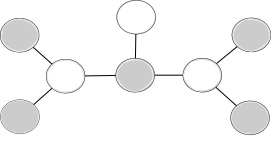
\includegraphics[scale=0.6]{images/greedy_fail.png}
	\caption{Greedy (5 nodos)}
\end{subfigure}
\begin{subfigure}[b]{0.4\textwidth}
	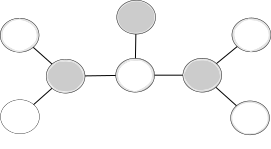
\includegraphics[scale=0.6]{images/greedy_best.png}
	\caption{Optimo (3 nodos)}
\end{subfigure}
\end{figure}

\begin{figure}[ht]
\centering
\begin{subfigure}[b]{0.4\textwidth}
	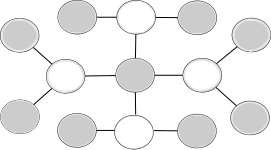
\includegraphics[scale=0.6]{images/greedy_fail2.png}
	\caption{Greedy (9 nodos)}
\end{subfigure}
\begin{subfigure}[b]{0.4\textwidth}
	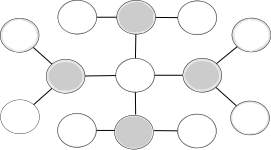
\includegraphics[scale=0.6]{images/greedy_best2.png}
	\caption{Optimo (4 nodos)}
\end{subfigure}
\caption{Ejemplos de nuestra heuristica comparado con el optimo.}
\end{figure}